% Figura 4 — a stack de observabilidade, toda ela na VM da API (ADR-009 e ADR-013).
\documentclass[11pt,tikz,border=6pt]{standalone}
\usepackage{fontspec}
\setmainfont{LibertinusSerif}[Extension=.otf, UprightFont=*-Regular,
  BoldFont=*-Bold, ItalicFont=*-Italic, BoldItalicFont=*-BoldItalic, Ligatures=TeX]
\setmonofont{Inconsolatazi4-Regular}[Extension=.otf, BoldFont=Inconsolatazi4-Bold,
  Ligatures=TeX, Scale=0.92]
\usetikzlibrary{arrows.meta,calc,fit,shapes.geometric}

\definecolor{tinta}{HTML}{1F2933}
\definecolor{petroleo}{HTML}{0F766E}
\definecolor{ambar}{HTML}{B45309}
\definecolor{fundo}{HTML}{F5F7F8}

\begin{document}
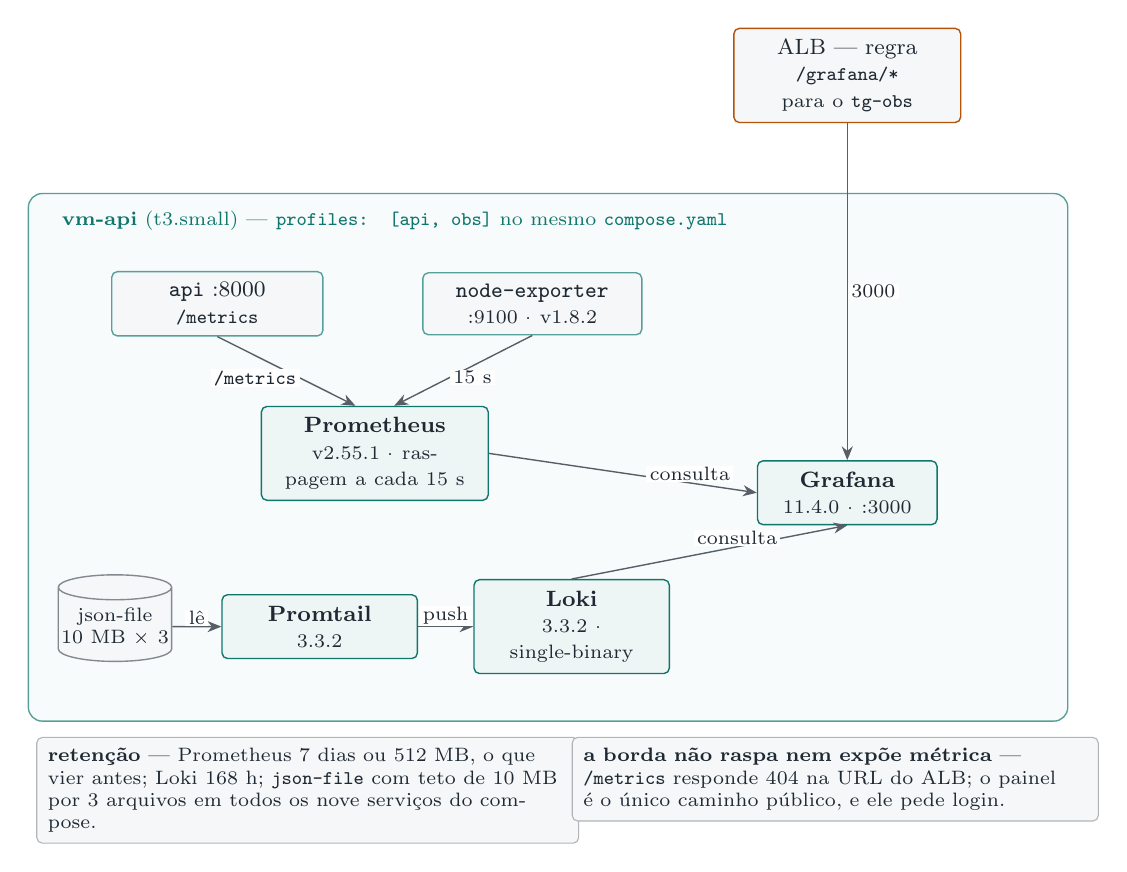
\begin{tikzpicture}[
    font=\footnotesize,
    >={Stealth[length=5pt,width=4pt]},
    caixa/.style={draw=petroleo, line width=0.5pt, fill=petroleo!7, rounded corners=2pt,
      align=center, inner sep=4pt, text=tinta},
    alvo/.style={draw=petroleo!70, line width=0.5pt, fill=fundo, rounded corners=2pt,
      align=center, inner sep=4pt, text=tinta},
    pub/.style={draw=ambar, line width=0.5pt, fill=fundo, rounded corners=2pt,
      align=center, inner sep=4pt, text=tinta},
    disco/.style={cylinder, shape border rotate=90, aspect=0.22, draw=tinta!55,
      line width=0.5pt, fill=fundo, align=center, inner sep=1pt,
      minimum height=1.1cm, minimum width=1.2cm, font=\scriptsize, text=tinta},
    nota/.style={draw=tinta!35, line width=0.4pt, fill=fundo, rounded corners=2pt,
      align=left, inner sep=4pt, text=tinta, font=\scriptsize},
    seta/.style={->, line width=0.5pt, draw=tinta!75},
    rot/.style={font=\scriptsize, text=tinta, fill=white, inner sep=1.2pt, inner ysep=0.5pt},
  ]

  % ---------- a VM que carrega a stack ----------
  \draw[draw=petroleo!70, line width=0.5pt, rounded corners=5pt, fill=petroleo!3]
    (2.2,0.8) rectangle (15.4,7.5);
  \node[font=\scriptsize, text=petroleo, anchor=north west] at (2.5,7.4)
    {\textbf{vm-api} (t3.small) — \texttt{profiles: [api, obs]} no mesmo \texttt{compose.yaml}};

  % ---------- alvos raspados ----------
  \node[alvo, text width=2.4cm] (api) at (4.6,6.1)
    {\texttt{api} :8000\\{\scriptsize \texttt{/metrics}}};
  \node[alvo, text width=2.5cm] (nodeexp) at (8.6,6.1)
    {\texttt{node-exporter}\\{\scriptsize :9100 · v1.8.2}};

  \node[caixa, text width=2.6cm] (prom) at (6.6,4.2)
    {\textbf{Prometheus}\\{\scriptsize v2.55.1 · raspagem a cada 15 s}};

  \node[disco] (logs) at (3.3,2.0) {json-file\\{\scriptsize 10 MB × 3}};
  \node[caixa, text width=2.2cm] (promtail) at (5.9,2.0)
    {\textbf{Promtail}\\{\scriptsize 3.3.2}};
  \node[caixa, text width=2.2cm] (loki) at (9.1,2.0)
    {\textbf{Loki}\\{\scriptsize 3.3.2 · single-binary}};
  \node[caixa, text width=2.0cm] (grafana) at (12.6,3.7)
    {\textbf{Grafana}\\{\scriptsize 11.4.0 · :3000}};

  % ---------- arestas ----------
  \draw[seta] (api.south) -- node[rot,left,pos=0.6] {\texttt{/metrics}} ([xshift=-7pt]prom.north);
  \draw[seta] (nodeexp.south) -- node[rot,right,pos=0.6] {15 s} ([xshift=7pt]prom.north);

  \draw[seta] (logs.east) -- node[rot,above] {lê} (promtail.west);
  \draw[seta] (promtail.east) -- node[rot,above] {push} (loki.west);
  \draw[seta] (prom.east) -- node[rot,above,pos=0.75] {consulta} (grafana.west);
  \draw[seta] (loki.north) -- node[rot,above,pos=0.6] {consulta} (grafana.south);

  % ---------- a borda ----------
  \node[pub, text width=2.6cm] (alb) at (12.6,9.0)
    {ALB — regra\\{\scriptsize \texttt{/grafana/*} para o \texttt{tg-obs}}};
  \draw[seta] (alb.south) -- node[rot,right] {3000} (grafana.north);

  % ---------- notas ----------
  \node[nota, text width=6.6cm, anchor=north west] at (2.3,0.6)
    {\textbf{retenção} — Prometheus 7 dias ou 512 MB, o que vier antes; Loki 168 h;
     \texttt{json-file} com teto de 10 MB por 3 arquivos em todos os nove serviços do compose.};
  \node[nota, text width=6.4cm, anchor=north west] at (9.1,0.6)
    {\textbf{a borda não raspa nem expõe métrica} — \texttt{/metrics} responde 404 na URL do ALB;
     o painel é o único caminho público, e ele pede login.};

\end{tikzpicture}
\end{document}
